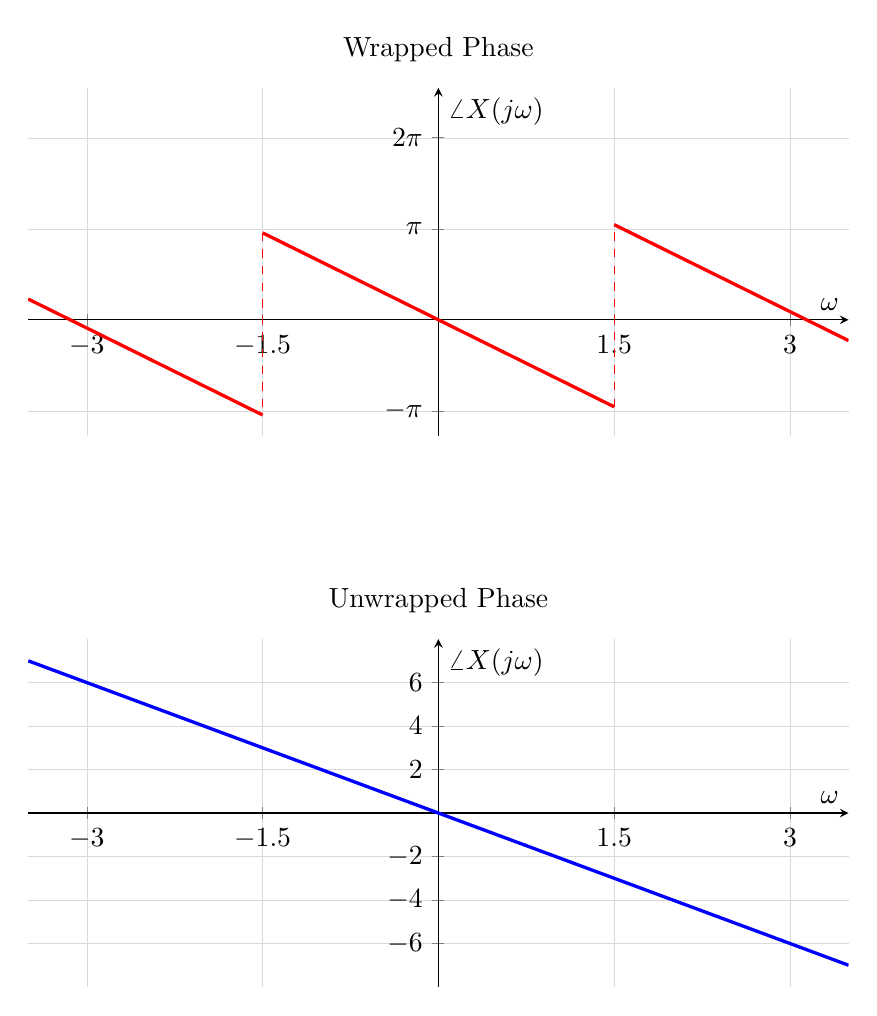
\begin{tikzpicture}
	% Define a common style
	\pgfplotsset{
		phase a/.style={
			width=12cm, height=6cm,
			axis lines=middle, xlabel={$\omega$},
			xmin=-3.5, xmax=3.5,
			xtick={-3,-1.5,1.5,3},
			grid=major, grid style={line width=.1pt, draw=gray!30},
			no marks,
		}
	}
	
	% Top plot: Wrapped Phase
	\begin{scope}[yshift=7cm]
		\begin{axis}[
			phase a,
			title={Wrapped Phase},
			ylabel={$\angle X(j\omega)$},
			ymin=-4, ymax=8,
			ytick={-3.14, 3.14, 6.28},
			yticklabels={$-\pi$, $\pi$, $2\pi$},
			]
			% Plot piecewise segments
			\addplot[red, very thick, domain=-3.5:-1.5] {-2*x - 2*pi};
			\addplot[red, very thick, domain=-1.5:1.5]  {-2*x};
			\addplot[red, very thick, domain=1.5:3.5]   {-2*x + 2*pi};
			
			% Mark discontinuities
			\draw[red, dashed] (axis cs:-1.5,3) -- (axis cs:-1.5,-3);
			\draw[red, dashed] (axis cs:1.5, -3) -- (axis cs:1.5, -3+2*pi);
		\end{axis}
	\end{scope}
	
	% Bottom plot: Unwrapped Phase
	\begin{scope}[yshift=0cm]
		\begin{axis}[
			phase a,
			title={Unwrapped Phase},
			ylabel={$\angle X(j\omega)$},
			ymin=-8, ymax=8,
			ytick={-6, -4, -2, 2, 4, 6},
			]
			\addplot[blue, very thick, domain=-3.5:3.5] {-2*x};
		\end{axis}
	\end{scope}
\end{tikzpicture}








